\documentclass{scu-thesis}
 \usepackage{graphicx}	% for including graphics
% \usepackage{amsmath}	% for advanced typesetting of mathematics
% \usepackage{txfonts}	% for using the Times-Roman font
% \usepackage{natbib}	% for better citation styles

\usepackage[letterpaper, portrait, margin=1in]
{geometry}

\geometry{	
lmargin = 1.25in,
rmargin = 1.25in,
}

\usepackage{graphicx}
\graphicspath{ {images/}}

\author{Eric Beckmann}
\author{Jonathan Coon}
\author{Mikael Figueroa}
\author{Matthew Voss}
\title{A Distributed Backup System}
\department{Department of Computer Science and Engineering}
\degree{Bachelor of Computer Science and Engineering}

% These must be set first ... the rest of the thesis commands rely on them.


% Only bachelor's theses should have multiple authors and/or be from
% multiple departments.  Signatures required:
%
% Bachelor's theses: advisor(s), department chair(s)
% Master's theses: advisor, reader, department chair
% Doctoral theses: doctoral committee (including advisor), department chair

\begin{document}
\frontmatter
\signature{Ahmed Amer}
\signature{Nam Ling}

\maketitle
\begin{abstract}
Backup systems are an important part of any IT infrastrucutre. They provide data assurance in the face of faulty hardware and software. Nonetheless, computer users commonly rely on backup systems that fail to exhibit either reliability, accessibility, security, or a combination of all three. We work to resolve this issue by creating a storage system in which users share encrypted data fragments amongst each other instead of with a single data storage entity. If data is corrupted on any single storage device, the data may be restored from a set of other storage devices.  Furthermore, this data is dispersed geographically. These architectural features of the sytem provide greater reliability and accessibility while the lack of any central service provider allows users to retain ownership of their data, improving privacy.
\end{abstract}

\include{Acknowledgements}

\tableofcontents
\listoffigures

\mainmatter
\chapter{Introduction}
Data loss is a fundamental, widespread problem in computing. In a single year, 25\% of PC users will lose their data. Furthermore, 100\% of all data storage technologies, ranging from magnetic tapes to hard drives to solid state storage, will inevitably fail. \footnotetext[1]{http://www.imagineiti.com/backup/biggest-backup-mistake/} Data loss is not only unavoidable, it is potentially devastating. 70\% of small businesses that experience major data loss go out of business in a year.\footnotemark[1] Moreover, the U.S. loses an estimated \$18.2 Billion every year due to data loss. \footnotetext[2]{https://gbr.pepperdine.edu/2010/08/the-cost-of-lost-data/} Almost every industry relies on accurately storing and accessing information, whether this be in the form of financial archives, software developmental codes, customer data, order records, etc. Backups, which are systems for duplicating one’s data and storing it in another place, counteract data loss.


\section{Motivation}
Many current solutions implement data backup. We observe, however, that all systems suffer problems with privacy, accessibility, resilience, or a combination of all three. Two general categories describe current solutions: enterprise backup, cloud backup and personal backup. Unfortunately, current enterprise solutions cannot be examined as they are often highly customized and proprietary. Cloud backup is a service in which users upload files to be stored in a data center. These systems, while they are highly redundant, are not immune to corporate problems. If the company providing your backups goes out of business, your backups will no long be accessible. In addition, these services may go down from time to time. Amazon S3, a common back end for such systems, has been known to have long outages \footnotetext[3]{https://gigaom.com/2008/07/20/amazon-s3-outage-july-2008/} \footnotetext[4]{http://www.rightscale.com/blog/cloud-industry-insights/amazon-ec2-outage-summary-and-lessons-learned/}. Personal backup, on the other hand, is the solution used by diligent individuals who regularly save their files to an external storage device or media. While personal backup addresses the privacy issue, the system is not resilient, since the external storage device will lose all the backup data if it ever fails \footnotetext[5]{https://www.backblaze.com/blog/hard-drive-reliability-stats-for-q2-2015/}. In addition, accessibility to the data relies on constant access to a single device.

\section{Solution}
Our backup system will address the issues of privacy, accessibility, and resilience. It will use redundancy and wide geographic distribution to create greater resiliency. We imagine at least one storage system per network. These storage systems will be interconnected, allowing them to share data. The data will be distributed as widely as the networks using these devices, encouraging hardware redundancy and making sure the data is constantly accessible. The protocol, once designed will be frozen, ensuring that these systems will continue to provide their services, even if support is no longer possible. Regarding privacy, we will not have access to the users' data, and each user's data will be only be accessible by the user who owns the data through encryption as mentioned above.

\chapter {Requirements}

We determined our requirements by consulting with Dr. Amer, our advisor who also acted as our customer.  All requirements are listed in order of importance for each section.  The ''Functional Requirements'' define what the system should do e.g. what actions it should enable and what services it should provide.  The ''Non-Functional Requirements'' define how the system should work and behave.  Often, non-functional requirements are qualitative attributes of the system.  The ''Design Constraints'' describe the real world limitations that our system needs to abide by.  Design constraints are very similar to non-functional requirement; however, where non-functional requirements are written in terms of the problem, design constraints are written in terms of the solution.

\section {Functional Requirements}

	\begin{itemize}
		\item The system must regularly and automatically create copies of a user's data and store the copies elsewhere for the purpose of backup.

		\item The system must, when prompted, restore that data from elsewhere back onto the computer.

		\item The system will have an interface for managing backup settings, such as choosing which files are backed up and how often the backup occurs.

		\item The system will only allow authenticated users to access its services.

	\end{itemize}

\section {Non-Functional Requirements}
	\begin{itemize}
		\item The system must avoid data loss.

		\item The system must allow data to be accessed at any time.

		\item The system will securely store data, preventing access from unauthorized parties and maintaining privacy.

		\item The system will widely distribute data to prevent a single point of attack by unauthorized parties.

		\item The system will have a user-friendly interface, hiding most of the complexity of data distribution from the user.

		\item The system will run transparently to the user, without noticeable performance reduction for the computer.
	\end{itemize}

\section {Design Constraints}
	\begin{itemize}
		\item The system must run on computers with Windows 7 and later.

		
	\end{itemize}
\section{Use Cases}
In this section, we will describe potential uses for our system. Backup systems have a fairily specific set of use cases, as seen in the following figure.

\begin{figure}[h]
\centering
\includegraphics[scale=0.5]{images/senior-design-user-model.png}
\caption{Use Cases}
\end{figure}

This backup product has a very specific set of use cases. Typical user sessions are listed below.

\subsection{Backing Up}
\begin{itemize}
	\item Principle Actor: An End User
	\item Pre-conditions:
\end{itemize}

\chapter{Activity Diagram}

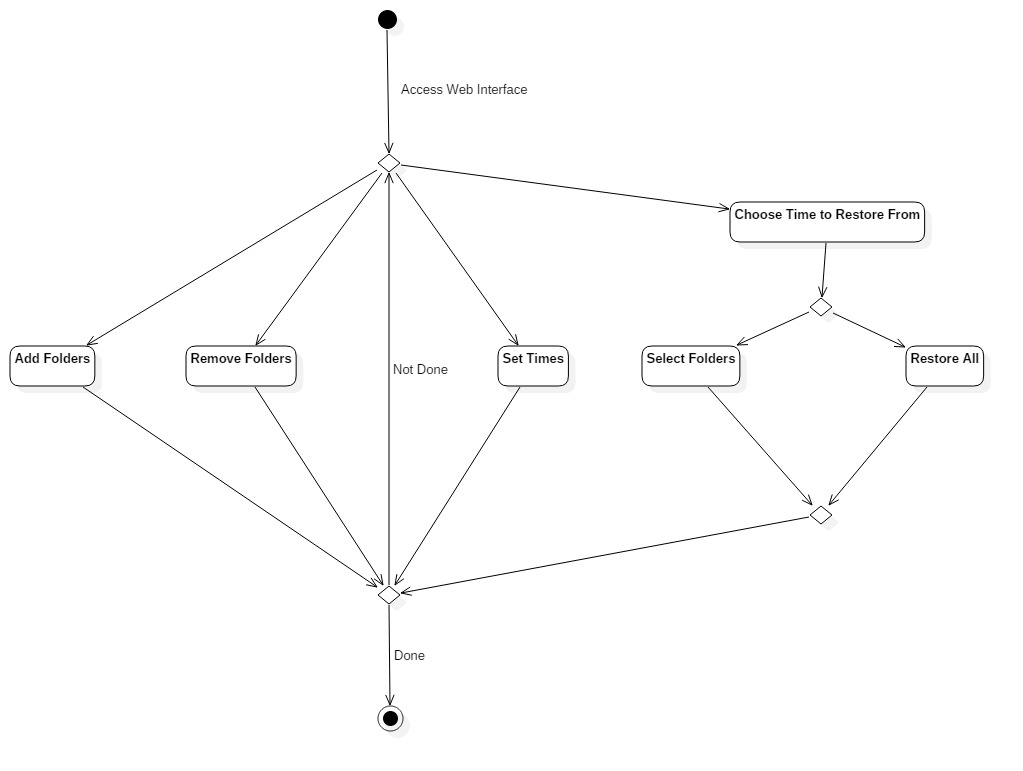
\includegraphics[scale=0.45]{images/ActivityDiagram1.jpg}
\chapter{System Architecture}


\section{Server to Server}

Figure \ref{fig:highLvlNetwork} details the overall, top-level view of our P2P network.  Our system is composed of a geographically distributed network of servers.  Each user or corporation which uses our network purchases one of these servers to place on their own LAN.  These servers work together to distribute and share data which has been backed up.  Even if one or multiple of the servers goes down, the data should be preserved due to the storage redundancy.

\begin{figure}[hb]
\centering
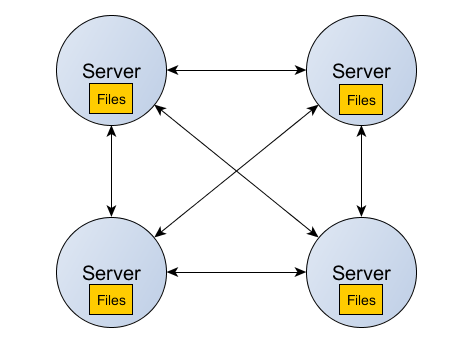
\includegraphics[scale=0.5]{images/architechure-diagram-server-server.png}
\caption{The highest level server-to-server system architecture}
\label{fig:highLvlNetwork}
\end{figure}

\clearpage


\section{Server to Client}

In the context of the local network of a single user, each of the client computers requiring data to be backed up
will connect to the server on that network. This server can be located anywhere within the network.
Upon the startup of each client, they each send a beacon to locate the server. The server and client
then make a connection and then secure it to allow the backup data to begin transferring. This relationship is reflected in Figure \ref{fig:indivNetwork}.

\begin{figure}[hb]
\centering
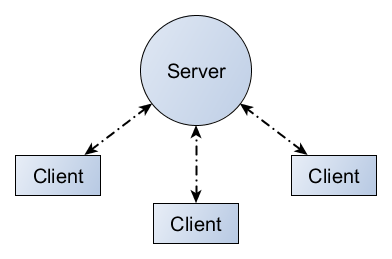
\includegraphics[scale=0.5]{images/architechure-diagram-server-client3.png}
\caption{The highest level server-to-server system architecture}
\label{fig:indivNetwork}
\end{figure}

\clearpage


\section{Server Architecture}

Figure \ref{fig:clientServer} details the internal structure of each individual server located on the user's LAN.  We see that each server has a connection into the larger P2P network of servers.  Also, each server connects to client machines on its LAN.  When a backup is initiated, either manually by a user or automatically according to scheduling, the Backup application on the server can start to retreive data from the client. Once the data and its form has been successfully stored, the Data Distributer is responsible for finding other backup servers and replicating the data to them.  When a user wishes to change the system's configuration, such as scheduling backup times or choosing which files to be backed up, they can access a Configuration web interface hosted on the server.  Finally, when the user wishes to restore, the Restore application is invoked, which takes data from the File Store and writes them back to the client.

\begin{figure}[hb]
\centering
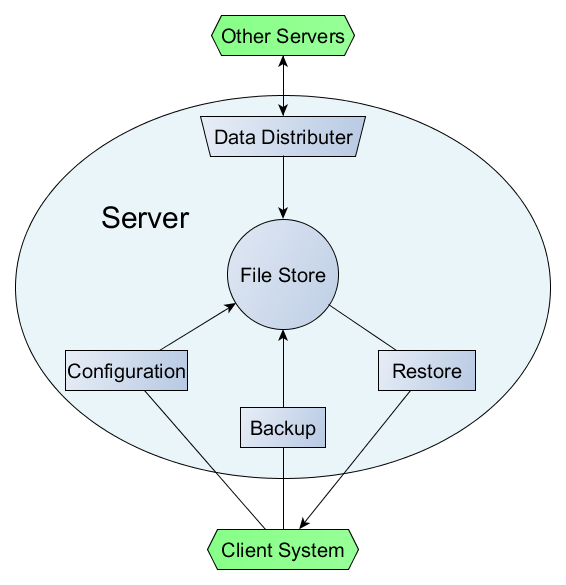
\includegraphics[scale=0.5]{images/architechure-diagram2.png}
\caption{A View of the Data Flow Through our Server}
\label{fig:clientServer}
\end{figure}
\chapter{Design Rationale}
	There are many reasons why we would make our system dual layer.  It makes sense that we have one layer for the client and another for the server box that each user has.  This allows alot of the systems activities to be transparent to the user, because they are happening on the external hardware and not on the user's own PC.  For example, all of the storage space is contained on this external box, as well as most of the distributed sending and receiving.

	Using OpenSSH to communicate between client and server allows the data transfers to be secure, and any listeners on the network should not be able to intercept anything.  The only vulnerable point is when the initial connection is made between the client and the server; however, through secure handshaking spoofing should be avoided.

	We will use MongoDB because it encapsulates and abstracts many common database functions for us, instead of requiring us to develop them ourselves.  It is well known and has been proven to function at a high performance level, with a good storage efficiency.
\chapter{Implementation}

\section{Storage}
Storage is the function of a backup system and we wanted to ensure that the storage mechanism we used would be reliable, secure, and maintainable. MySQL was a clear choice. It is well tested, contains an excellent permissions system, and is commercially supported. 
\subsection{Storage Layout}
Internally the database uses five different tables to store all data: clients, jobs, files, blocks, and logs. The "clients" table relates the IP address of the client to a client ID. The "jobs" table relates a job ID  with a time and a client. The file table relates file permissions and dates to a file ID. The blocks table stores all the file data in a series of blocks which are indexed by their SHA1 hash.

In order for the structure of the file system to be properly represented, we needed a way to relate files to each other to form a directed tree. This is provided by a file table that relates one file ID to another. While this table is sufficient to represent a graph of files, the file systems we back up are proper trees. Using this system has an added benefit: Files and directories can be represented using the same schema. Since both have identical collection of attributes, we use this system without any loss of information.

Jobs need to be related to a series of files to be backed up on the client machine. To do this, a table relating file IDs to job IDs is provided. As many file IDs as desired can be related to a given job ID.

The actual data contained in the files are stored in a table of blocks. Each block is of a fixed size and is indexed by its hash. The file metadata is related to a set of blocks through an intermediate table that relates file IDs to the hashes of the blocks that make up the file. The entries are inserted in the order that the blocks appear in the file.

\subsection{Storage Optimization}
Separating files into blocks allowed us to optimise the storage used. Many files share common parts, and duplicate blocks are simply not inserted into the system. In our tests, we got up to 30% compression on par with the GZIP compression algorithm.
\subsection{Insertion}
Once a client has been inserted, a job has been created, and the job has been related to the directories the user wants to back up, the inserter uses the SFTP protocol to connect to the client system at the IP stored in the clients table. It logs into the system using a predefined password. It then recursively compares the record for each directory, updating file entries that already exist and inserting file records that do not exist. No file record is ever deleted.

\section{Distribution Algorithm}

In order to distribute the backup data across our network, our system uses a
peer-to-peer networking algorithm based on Content Addressable Networks. \cite{scalable}
The algorithm is centered around the concept of a hash table that is shared by all the backup
servers in the network. The hash table is modeled as a square, and the backed up files are then
points that are hashed into this square. Each backup server in the network owns a rectangular portion
of this square, and is responsible for storing all the files whose points map into this rectangle.
This concept is shown in Figure \ref{fig:dht_1}. In this figure, in order to retrieve file 8 from the server,
it has to be retrieved from backup server 2.

\begin{figure}[hb]
\centering
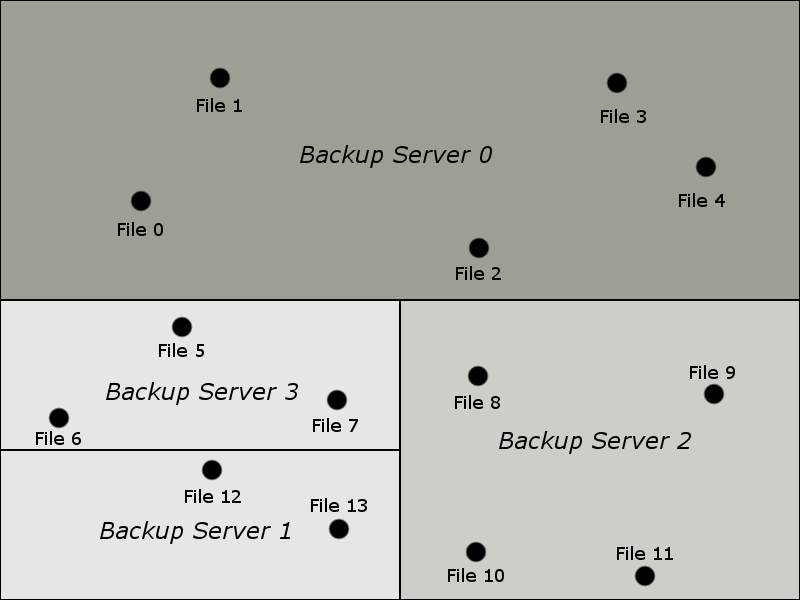
\includegraphics[scale=0.5]{images/dht_basic.png}
\caption{Distributed Hash Table}
\label{fig:dht_1}
\end{figure}

This algorithm has to take into account the fact that the network is chaotic and unstable.
Any backup server within the network can disappear from the network at any time and without warning.
Any backup server can also rejoin the network at any time. This is accounted for by the algorithm by
the way the network is structured. Each backup server in the network only communicates directly with
other servers that own a portion of the hash table adjacent to its own portion, called its neighbors.
For example, in Figure \ref{fig:dht_2}, backup server 2's neighbors are servers 4, 9, 3, and 8.

\begin{figure}[hb]
\centering
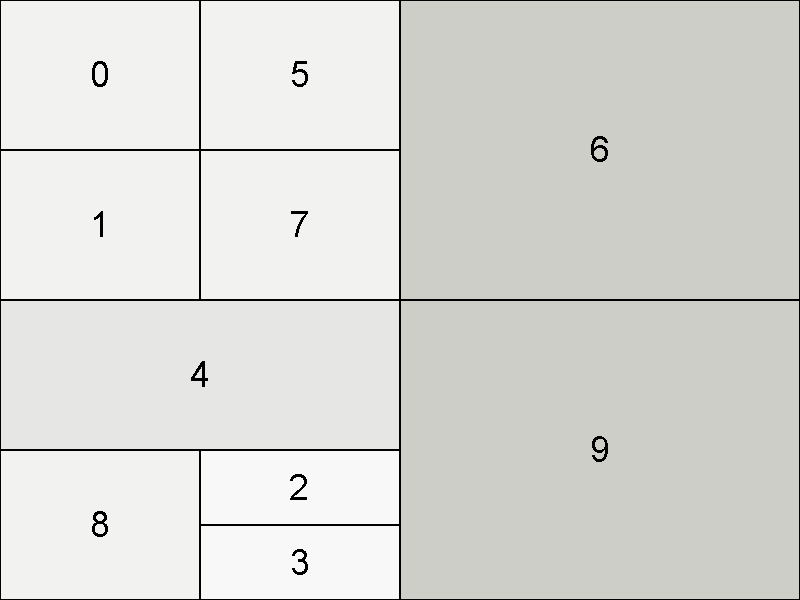
\includegraphics[scale=0.5]{images/dht_10_nodes.png}
\caption{Distributed Hash Table with 10 nodes}
\label{fig:dht_2}
\end{figure}

Then in order to deal with the fact that a backup server could disappear from the network at any time,
the neighbors of a backup server that goes down are responsible for taking over the space it occupied
in the hash table. Each backup server maintains consistent communication with its neighbors. If a server
is no longer responding to its neighbors, then those neighbors will negotiate to see who takes ownership
of the space the unresponsive server occupied in the hash table. In this way, each backup server is responsible
for maintaining the stability of the network near it in the hash table.
 


\section{Client-Server Discovery Procedure}
\begin{figure}
\centering
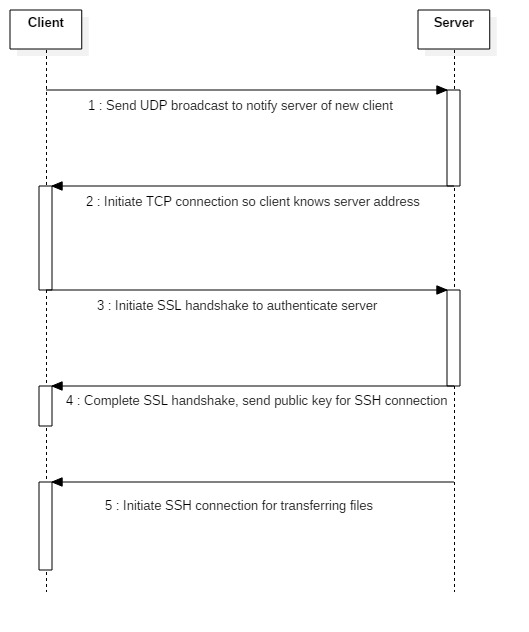
\includegraphics[scale=0.5]{images/SequenceDiagram1.jpg}
\caption{Client-Server Discovery Procedure}
\label{fig:connect}
\end{figure}

Once the user has already set up the server on their own LAN, they are ready to connect their own client machines to the system.  The user installs certain basic client software on their machine which, upon activation, sends out a UDP broadcast onto the network to notify the server of a new client.  Once the server receives the broadcast, it then initiates a TCP connection so that the client knows the proper server address to connect to.  The client then initiates an SSL handshake using the wolfSSL library, in order to verify that the server is a valid party and not just a listener on the network who wishes to intercept data.  This is made possible by each server possessing it's own unique private key, set at manufacture time, and signed by our central certifiate authority  The client program includes a public key that can verify that the server is who it says it is.  Once the ssl handshake is completed, the server sends a public key to the client which the client can use to recognize a legetimate openSSH connection.  In addition, at this point the client is given a private key used by the server to identify its unique user account for accessing files.  Now that both the client and the server possess valid credentials and information on each other, the server may then initiate ssh connections for transferring files.

\section{Web Configuration Interface}

Our Web Configuration Interface was a simple webpage, and so used the typical technologies of HTML, Javascript, and PHP.  IgniteUI was used to construct the interface.  PHP extensions were used to call various applications on the server in response to user inputs.
\chapter{Testing Plan}

The purpose of this system is to provide a secure, private, efficient, reliable, and constantly accessible data backup system.  Therefore, any failures could be critical, possibly causing people or corporations to lose their data and resulting in millions of dollars in damages.  It is our responsibility to ensure that each individual component of the system works perfectly, and also that the system as a whole smoothly functions.

Since our intended system is very complex and consists of several modules, we will most likely follow an incremental process model, and use the continuous integration approach.  Under this method, performing unit testing is very intuitive, as each team member will continuously test their own modules in isolation as they develop them.  We will remember to test early and often in order to catch bugs as soon as possible.  Part of this will be white box testing for code coverage; at the very least, we should make sure all  linearly independent paths through the code are tested.  Furthermore, we will make careful documentation of all bugs we catch.  This practice will help us get a better idea of common failure points in our modules, so we can focus more on those areas when we test later on.  At least once per month, we will peer-review each others' modules in order to ensure good coding practices, including high cohesion and low coupling.  Once we have a working system, we will perform black box testing with team members using the system for their own personal backups, and sharing files amongst the four of us.

Besides testing within the team, we should also open testing up to focus groups representing hypothetical users.  Once our system reaches a fully-working version, we will find friends and family members to try using our system.  The obvious problem is that we cannot ask them to rely fully on our system as a replacement to the backup systems they already use, because if our system fails that will represent a great inconvenience and loss to them.  Therefore, we will ask them to use our system in addition to whatever backups they currently use.  Our final system relies on a large network of users sharing files with each other using a peer-to-peer protocol; therefore at some point we should open the system up to the general public for beta testing.  Once again, we must put a disclaimer as clearly as possible that this system cannot yet guarantee privacy and reliability.  A public beta testing would definitely require the most effort to implement and maintain, but it will be necessary before we can release any type of product.  We may not reach this phase in the course of this year, but if we continue the project later we definitely will.
\chapter{Risk Analysis}

\hspace*{-2cm}
\begin{tabular}{p{5cm} | p{3cm} | l | l | l | p{4cm}}
\hline

Risk & Consequences & Probability & Severity & Impact & Mitigation Strategy \\

\hline

Insufficient testing.  Our project is a massively distributed system theoretically containing thousands of users.  Fully testing in this context will require massive automation and virtualization, and we may not be able to set up that infrastructure. & Our system will not be fully tested and may have many bugs. & 0.7 & 5 & 3.5 & We will come up with smaller scale tests that will simulate a larger environment. \\

\hline

Our team may not be able to develop an optimal data distribution algorithm in time.  This is the most innovative and research intensive part of the project, and we may not be able to complete it. & Our system, while working, will not be optimal or innovative. & 0.5 & 6 & 3.0 & All team members must start researching this part of the system early and also constantly brainstorm and share ideas so that our maximum innovation potential is reached. \\

\hline

Our team makes a repository error that breaks the project with no simple way of recovery & We may lose commit information, meaning we will have to redo work and also spend more time to fix the repository. & 0.4 & 7 & 2.8 & We will practice good repository techniques such as each person developing on their own branch and carefully reviewing changes before merging them. \\

\hline

\end{tabular}
\hspace*{-2cm}
\chapter{Development Timeline}

\begin{figure}[h]
	\centering
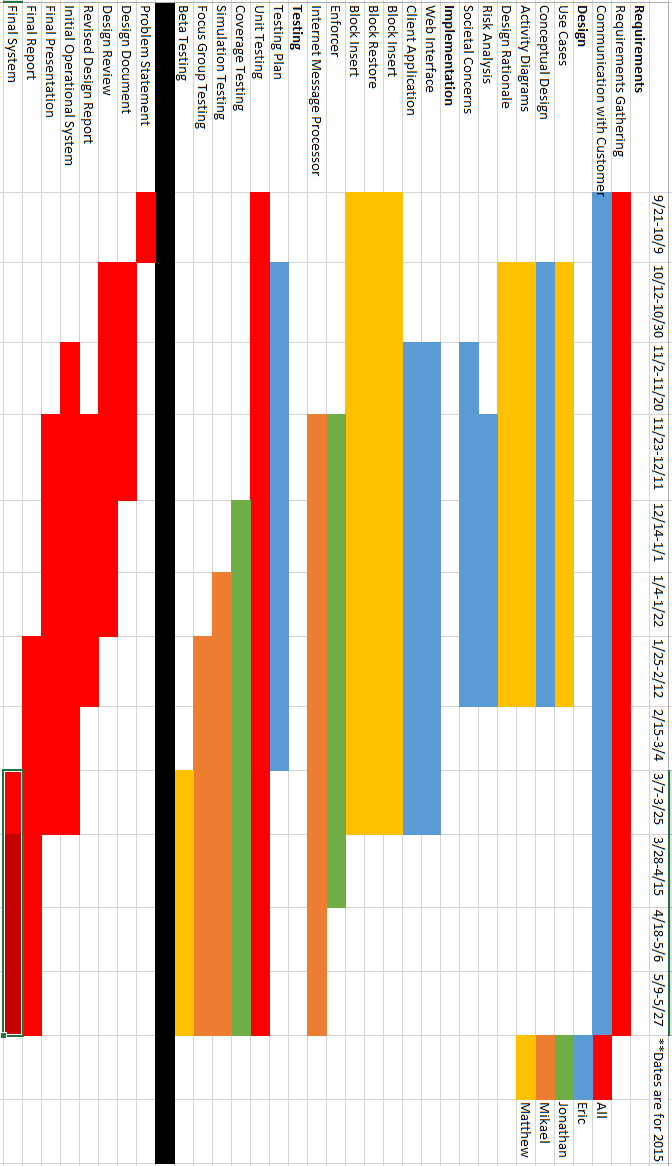
\includegraphics[scale=0.90]{images/GANT.png}
	\caption{GANT chart}
	\label{fig:gant}
\end{figure}
\chapter{Societal Issues}

\section{Ethical Discussion, Social Concerns, and Compassion}

\subsection{Justification}
	There are many ethical justifications for our project.  In the larger sense, we hope to make the world a better place by providing a better data backup and restore service than what is currently out there.  The bottom line is that our product will provide a convenience to the general public and assist them with storing files and also protecting against the problems of data loss.  Specifically we will help corporations become more efficient in their operations, which could bring economic prosperity and higher standards of living for society as a whole.  This is all in agreement with the first rule of the ACM Code of Ethics to ''contribute to society and human well-being.'' \cite{acmethics}

	Our project also deals directly with the human right to privacy.  As detailed in rule 1.7 of the ACM code of ethics, we are to ''respect the privacy of others.'' \cite{acmethics}  Furthermore, privacy is listed as a fundamental human right in Article 12 of the Universal Declaration in Human Rights: ''no one shall be subjected to arbitrary interference with his privacy.'' \cite{udhr}  The right to privacy is an inalienable human dignity that we hope to protect.  Privacy is so important because it gives people greater freedom to make their own moral decisions, independent from the judgement of others and shielded from the pressure to conform to their culture.  As one adage goes: ''The time you spend alone with yourself is the most precious time you have.  This is your proving ground.  It’s where you decide who you are, what values you uphold, and ultimately how you are seen in the eyes of yourself and others.'' \cite{wolf}

	The right to privacy is especially pertinent in this day and age, where more and more of everyone’s personal data is being put out online, vulnerable to access by malicious parties.  We hope our service will allow people to protect their privacy, since instead of storing their data in a single corporation’s database, which presupposes full trust in that corporation, and also provides a single point of attack for governments or hackers who wish to seize the data, we will be distributing the encrypted data securely to many locations in separate fragments.  These are not merely hypothetical concerns.  Data stores run by single entities have suffered data breaches many times in the past.  For example, Apple iCloud was hacked in August of 2014, which resulted in many celebrity photographs being leaked. \cite{independent}  Furthermore, the NSA has controversially forced companies like Google and Yahoo to turn over customer data in moves that have widely been called unconstitutional. \cite{gizmodo}  Our system will not be vulnerable to privacy violations like this, because there will no longer be a single party attackers can go after to view people's data.

\subsection{Lifelong Learning}

	Throughout this project, it is also very important that we are mindful of our own growth in moral character and technical skill.  Our society is increasingly dependent on computers, so as computer engineers we have a large role for improving people’s daily lives.  As we go through this project, we will be sure to adhere to the Software Engineering code of ethics.  We will make every effort to put the public interests and the common good first.  We will strive for the highest quality work in all aspects.  We will strive to cultivate our own character, skills, and abilities, and will seek to grow as much as possible through this project.  Finally, we will treat each other with respect during this project.

\subsection{Possible Pitfalls}
	As with most engineering projects, there are certain moral pitfalls that we might encounter along the way.  First of all, we have to consider that potential users of our system are trusting us to keep their data as private as possible.  If we take any shortcuts or make any oversights while designing our system, we could leave security holes that will compromise privacy.  By not keeping people's data private, we expose them to malicious parties such as idenity thieves, hackers, fraud artists, and so on.  We would be indirectly responsible for any damage caused, because we made people believe they had privacy which they did not.  And this would break article 1.7 of the ACM Code of Ethics to ''Avoid harm to others''. \cite{acmethics}  It is therefore our duty to ensure privacy in our system to the maximum extent possible.

	There is also the possible pitfall of our system being used by criminals, due to the enhanced privacy it provides.  By providing a system by which users can store their data with complete privacy, we could allow criminals to hide evidence of their activities, obstructing the activities of legitimate law enforcement agencies. The peer-to-peer architecture we use is similar to protocols such as BitTorrent which are far and wide used only for illicit purposes.  Even though it is not our intention that our system would be used for illegal activities, we must consider this possibility.

\section{Political Concerns}
	This is not a public project, so we can mostly disregard political concerns.

\section{Economic considerations and Manufacturability}
	The scope of the project at this stage is not to deploy a large scale product for the public to use, but rather to make a system for the purposes of testing new algorithms and methods of data distribution.  Therefore, we will not consider the costs of deploying a final product at this time.

	As for the costs of prototyping itself, we expect it to be quite low.  The software development costs little to no resources.  We will use a number of Raspberry Pi boards to implement our system.  At the cost of \$40 per board, we expect the total cost of the project to be no more than \$300.  We will support this project with our own personal funds.

\section{Health and Safety}
	This project does not require the use of any heavy machinery, extraordinarily large power sources, etc.  Therefore, we don't need any special safety considerations for this project.  However, we will be using electronic equipment such as PCs and Raspberry Pis in the course of this project, so we should exercise common sense as we would handling any electronic appliance.

\section{Sustainability and Environmental Impact}
	The environmental impact of creating our starting system should be minimal, since it is quite small scale and only uses a few electronic devices.  For the reasons mentioned above we will not yet consider the costs of deployment for a large scale system.

\section{Usability}
	One of the requirements and goals for our system is to make our interface as user-friendly as possible.  We will do this by only providing our user with a basic set of controls, hiding the complexity of the data distribution algorithm from them.  It is also important that our system be easy to set up as well.  We can acheive this by making a good installer as well as utilizing auto-configuration to the fullest extent.  Finally, we will do our utmost to prevent hogging of system resources by our program, so that it runs as transparently in the background as possible.
\chapter{Conclusion}
\section{Lessons Learned}


Another challenge we had to learn to overcome was poor documentation in the third-party libraries we used.  In the course of this project, we had to use many libraries in multiple operating system environments.  Many of these libraries were openly sourced and developed by third-parties.  For example, we used IgniteUI for the design of the web interface, WolfSSL for the secure handshake in the discovery procedure, and OpenSSH for the file transfer.  Unfortunately, most of these libraries had poor documentation, providing very little description as to their usage, and sometimes even giving contradicting information.  The lesson we learned from this challenge was to take into account the difficulty in diciphering the usage of third-party libraries when deciding whether or not to use them.  Furthermore, we learned techniques for deducing the usage of libraries.  For example, some libraries had similar function patterns as common libraries we had all encountered before, allowing us to infer the proper usage.

%\bibliography{master}
%\bibliographystyle{ieee}

\begin{thebibliography}{9}

\bibitem{acmethics}
Acm.org, 'Code of Ethics            —                Association for Computing Machinery', 2015. [Online]. Available: http://www.acm.org/about/code-of-ethics. [Accessed: 30- Nov- 2015].

\bibitem{imagineiti}
Imagine IT, Inc., 'Biggest Backup Mistake - Minneapolis, St Paul, Edina| Imagine IT, Inc.', 2015. [Online]. Available: http://www.imagineiti.com/backup/biggest-backup-mistake. [Accessed: 30- Nov- 2015].

\bibitem{wolf}
Imgur, 'The time you spend alone with yourself.', 2015. [Online]. Available: http://imgur.com/gO8Xiot. [Accessed: 30- Nov- 2015].

\bibitem{udhr}
Un.org, 'The Universal Declaration of Human Rights | United Nations', 2015. [Online]. Available: http://www.un.org/en/universal-declaration-human-rights/. [Accessed: 30- Nov- 2015].

\bibitem{theguardian}
C.  Arthur, 'Naked celebrity hack: security experts focus on iCloud backup theory', the Guardian, 2014. [Online]. Available: http://www.theguardian.com/technology/2014/sep/01/naked-celebrity-hack-icloud-backup-jennifer-lawrence. [Accessed: 30- Nov- 2015].

\bibitem{gizmodo}
A.  Estes, 'Confirmed: NSA Paid Google, Microsoft, Others Millions for PRISM Aid', Gizmodo, 2015. [Online]. Available: http://gizmodo.com/confirmed-nsa-paid-google-microsoft-others-millions-1188615332. [Accessed: 30- Nov- 2015].

\bibitem{dropbox_fail}
A.  Ferdowsi, "Yesterday's Authentication Bug", Dropbox Blog, 2011.

\bibitem{khaaaaan}
Khan, J.I.; Tahboub, O.Y., "Peer-to-Peer Enterprise Data Backup over a Ren Cloud," in Information Technology: New Generations (ITNG), 2011 Eighth International Conference on , vol., no., pp.959-964, 11-13 April 2011.

\bibitem{backblaze}
A.  Klein, 'The Most Reliable Hard Drive 2015', Backblaze Blog | The Life of a Cloud Backup Company, 2015. [Online]. Available: https://www.backblaze.com/blog/hard-drive-reliability-stats-for-q2-2015/. [Accessed: 30- Nov- 2015].

\bibitem{independent}
M.  Landi, 'Stars' nude photo attack may have been down to password codes - Independent.ie', Independent.ie, 2014. [Online]. Available: http://www.independent.ie/business/technology/news/stars-nude-photo-attack-may-have-been-down-to-password-codes-30552629.html. [Accessed: 30- Nov- 2015].

\bibitem{hp}
M.  Lillibridge, S.  Elnikety, A.  Birrell and M.  Burrows, "A Cooperative Internet Backup Scheme", Usenix, 2003.

\bibitem{gigaom}
O.  Malik, 'S3 Outage Highlights Fragility of Web Services', Gigaom.com, 2008. [Online]. Available: https://gigaom.com/2008/07/20/amazon-s3-outage-july-2008/. [Accessed: 30- Nov- 2015].

\bibitem{scalable}
S.  Ratnasamy, P.  Francis, M.  Handley, R.  Karp and S.  Schenker, "A scalable content-addressable network", ACM SIGCOMM Computer Communication Review, vol. 31, no. 4, pp. 161-172, 2001.

\bibitem{multiagent}
Shibakawa, M.; Uchiya, T.; Takumi, I.; Kinoshita, T., "Design and implementation of multiagent-based distributed backup system," in Computer and Information Science (ICIS), 2013 IEEE/ACIS 12th International Conference on , vol., no., pp.235-240, 16-20 June 2013.


\bibitem{pepperdine}
D.  Smith, 'The Cost of Lost Data', Graziadio Business Review, vol. 6, no. 3, 2003.

\bibitem{password}
Taneski, V.; Hericko, M.; Brumen, B., "Password security — No change in 35 years?," in Information and Communication Technology, Electronics and Microelectronics (MIPRO), 2014 37th International Convention on , vol., no., pp.1360-1365, 26-30 May 2014.

\bibitem{uchiya}
Uchiya, T.; Shibakawa, M.; Takumi, I.; Kinoshita, T., "Multiagent-based distributed backup system for individuals," in Computer and Information Science (ICIS), 2015 IEEE/ACIS 14th International Conference on , vol., no., pp.361-366, June 28 2015-July 1 2015.

\bibitem{rightscale}
T.  Von Eicken, 'Amazon EC2 Outage: Summary and Lessons Learned', Rightscale.com, 2011. [Online]. Available: http://www.rightscale.com/blog/cloud-industry-insights/amazon-ec2-outage-summary-and-lessons-learned/. [Accessed: 30- Nov- 2015].

\bibitem{syncthing}
Available: https://syncthing.net/.

\bibitem{crashplan}
Available: http://www.code42.com/crashplan/.

\end{thebibliography}

\backmatter
\end{document}
